\chapter{Auswertung Benchmark}
Im folgenden werden die Ergebnisse des Benchmarks ausgewertet.
Dazu wird zu erst die Gesamtlaufzeit des Benchmarks in \autoref{auswertung:generell} analysiert. Dabei wird zwischen zeilenbasierten und spatenbasierten
Tabellen unterschieden.
Anschließend wird in \autoref{auswertung:queries} auf die Laufzeit der
einzelnen Unterabfragen des Benchmarks eingegangen.
Dabei soll untersucht werden welche Abfragen besonders schnell sind.
In \autoref{auswertung:basic_indizes} und \autoref{auswertung:hardware}
wird der Einfluss von Indizes bzw.\ unterschiedlicher Hardwarekonfigurationen
untersucht.

\section{Gesamtlaufzeit des Benchmarks}\label{auswertung:generell}

\begin{tabularx}{\textwidth}{Xrr}
	\toprule
	 & \textbf{Rowstore} & \textbf{Columnstore}\\
	\midrule
	\endhead
	\hline
	\caption{Gesamtlaufzeiten von Row- und Columnstore in usec}
	\label{auswertung:gesamtlaufzeit}
	\endfoot
	Durchschnitt & 754689 & 3591003 \\
	Minimum & 725710 & 3451791 \\
	Maximum & 858595 & 4079505 \\
	Median & 752236 & 3577376 \\
	Standardabweichung & 17619 & 79002\\
	Gesamt & 754689 & 3591003 \\
\end{tabularx}

Allgemein sollten Benchmarks auf der HANA Datenbank immer zwischen
Row- und Columnstore unterscheiden.
Dies wird deutlich beim Betrachten der Allgemeinen Laufzeit.
Wie \autoref{auswertung:gesamtlaufzeit} zu entnehmen ist, besteht ein deutlicher
Unterschied in der Laufzeit zwischen Row- und Columnstore.
Da der SSBM Benchmark als Maß für Abfragen im Bereich des Datawarehouse
eingesetzt wird, kann also allgemein gesagt werden,  dass der Columnstore
dem Rowstore im Datawarehouse Umfeld vorzuziehen ist.
Jedoch sollte bedacht werden, dass es sich bei dem SSBM Benchmark um
reine Abfragen von Daten handelt. Wie in \autoref{row_col:rowstore} beschrieben
kann ein Rowstore von Vorteil sein, wenn Daten gespeichert werden.

\begin{figure}[H]
	\centering
	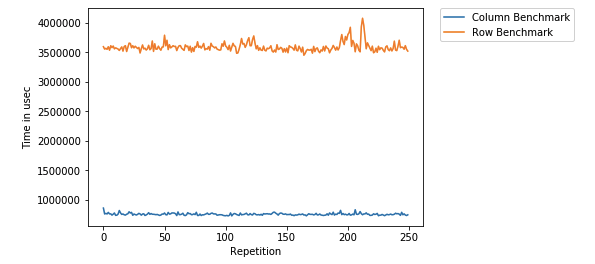
\includegraphics[width=0.7\textwidth]{images/performanceentwicklung.png}
	\caption{Gesamtlaufzeit von Row- und Columnstore}\label{auswertung:gesamtlaufzeit:graph}
\end{figure}
Anhand der Standardabweichung und \autoref{auswertung:gesamtlaufzeit:graph} ist auch zu sehen, dass der Columnstore
eine konstantere Zeit pro Abfrage aufweist.
Allerdings da der Rowstore im allgemeinen langsamer ist als der Columnstore
kann dies vernachlässigt werden, da die Standardabweichung relativ zur
Gesamtlaufzeit sehr gering ist.

\section{Vergleich der SSBM Queries}\label{auswertung:queries}

Im folgenden wird die Laufzeit einzelner Queries des SSBM Benchmarks separat betrachtet.
Dazu wird der Benchmark in die Gruppen Q1, Q2, Q3 und Q4 unterteilt.
Diese Gruppen bestehen aus einzelnen Unterabfragen Q1.1, Q1.2 etc.
Zuerst wird allgemein die Geschwindigkeit der einzelnen Gruppen verglichen
und anschließend auf ausgewählte Unterabfragen eingegangen.

\begin{figure}[H]
	\centering
	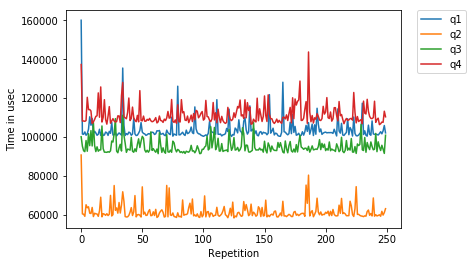
\includegraphics[width=0.49\textwidth]{images/Analysis-SSBM-HANA_18_0.png}
	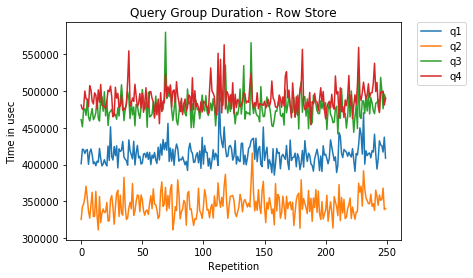
\includegraphics[width=0.49\textwidth]{images/Analysis-SSBM-HANA_23_0.png}
	\caption{Query-Gruppen Laufzeit}\label{auswertung:query-group}
\end{figure}

In \autoref{auswertung:query-group} ist zu erkennen, dass die
Laufzeit einzelner Queries durch zeilenbasiete bzw. spaltenbasierte
Tabellen beeinflusst wird. Zwar sind allgemein die spaltenorientierten Tabellen
deutlich schneller, jedoch ist Q3 bei spaltenorientierten
Tabellen schneller als Q1, wohingegen bei zeilenorientierten Tabellen
Q1 schneller als Q3 ist.
Gleich bleibt, dass Q2 die schnellsten und Q4 die langsamsten Queries sind.
Um zu verstehen wodurch der Unterschied von Q1 und Q3 zustande kommt wird
im folgenden der jeweils die Unterabfragen von Q1 und Q3 im Row store betrachtet.
Anschließend werden die selben Queries im Row store betrachtet und
dann verglichen.

Da der SSBM Benchmark so gestaltet ist dass die Queries
von Q1 nach Q4 immer komplizierter werden ist es verwunderlich,
dass Q3 schneller als Q1 ist.
Dazu werden in \autoref{auswertung:comp:q3} und \autoref{auswertung:comp:q1}
die Unterabfagen von Q3 betrachtet.

\begin{figure}[H]
	\centering
	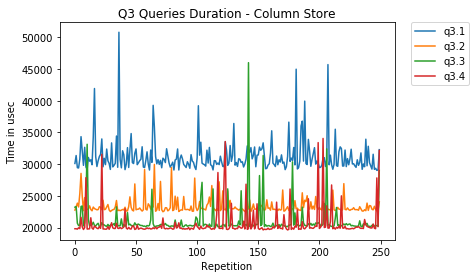
\includegraphics[width=0.49\textwidth]{images/q3-col.png}
	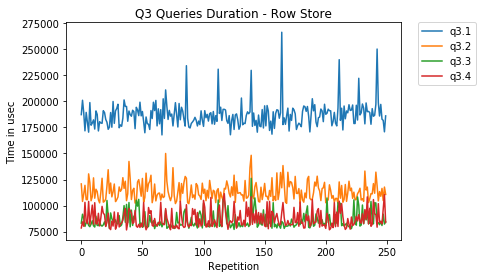
\includegraphics[width=0.49\textwidth]{images/q3-row.png}
	\caption{Q3 Vergleich Row vs Column}\label{auswertung:comp:q3}
\end{figure}

Aus \autoref{auswertung:comp:q3} lässt sich erkennen, dass Q3.1 sich relativ
zu Q3.2, Q3.3 und Q3.4 verbessert hat.
Um dies zu versehen werden im folgenden der Executionplan zu Q3.1 des Columnstores
und des Rowstores verglichen, welche in \autoref{auswertung:q3.1:col} und 
\autoref{auswertung:q3.1:row} im Anhang zu finden sind.
Beim Vergleich der Executionpläne wird deutlich dass der Columnstore dabei
einen Filter auf 4 Tabellen durchführt.
Dies ermöglicht eine Parallelisierung der Abfragen,
wohingegen beim Rowstore diese Parallelisierung nicht möglich ist.

\begin{figure}[H]
	\centering
	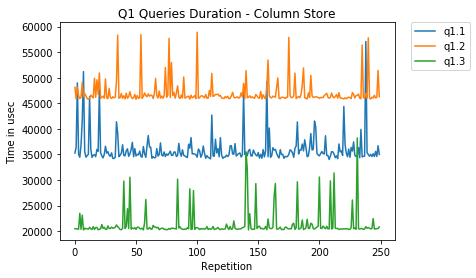
\includegraphics[width=0.49\textwidth]{images/q1-col.png}
	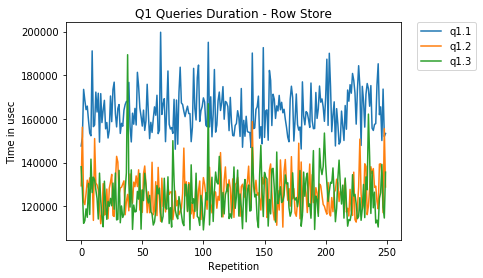
\includegraphics[width=0.49\textwidth]{images/q1-row.png}
	\caption{Q1 Vergleich Row vs Column}\label{auswertung:comp:q1}
\end{figure}

%TODO
% Vergleich von q1, q2, q3, q4 etc.
% Diagramm
% Welche ist die schnellste und warum?
% Stabilität einzelner Queries

\section{Einfluss der grundlegenden Indizes}\label{auswertung:basic_indizes}
%TODO
% Row with or without indices
% Column with or without indices

\subsection{Grundlegende Untersuchung für Column-Store}

\begin{table}[H]
\centering
    \begin{tabularx}{10cm}{lrrr}
        \toprule
        Merkmal             &   Col[ms]    &    Col Index[ms] & Abweichung[\%]\\
        \toprule
        Samples             &   250        &   250      &        \\
        \midrule    
        Max                 &   859        &   697      & -18.8\%\\
        Min                 &   726        &   546      & -24.7\%\\
        Median              &   752        &   574      & -23.6\%\\
        Average             &   755        &   578      & -23.4\%\\
        Standard Deviation  &   18         &   19       & +5.5\%\\
        Total               &   188672     &   144605   & -23.3\%\\
        \bottomrule
    \end{tabularx}
\caption{Vergleich der Ergebnisse mit und ohne grundlegende Indizes für Column-Store.}
\label{tab:basic_index_col}
\end{table}

Durch hinzufügen der grundlegenden Indizes wurde der Benchmark
für Columstores sowohl im Schnitt als auch im Median schneller.
Im Schnitt wurde er 23,4\%, im Median um 23,6\% schneller.
Die Standardabweichung hat sich jedoch nur geringfügig verändert.
Die Werte streuen relativ gesehen also gleich stark wie zuvor.
Folglich konnten Mindest- und Maximallaufzeit auch deutlich reduziert werden. 


Diese Ergebnisse sind interessant,
da Columnstores bereits einen natürlichen Index
durch speichern der Daten in Spalten haben,
wie in \autoref{sec:col_store} beschrieben.
Deshalb profitieren Columnstore meist nicht von zusätzlichen Indizes.
Um herauszufinden, warum trotzdem eine deutliche Verbesserung merkbar ist,
wird der Query-Execution Plan des Subqueries mit der deutlichsten Verbesserung
im folgenden untersucht.

\subsubsection{Untersuchung der Laufzeit für einzelne Query-Gruppen}

\begin{table}[H]
    \centering
    \begin{tabularx}{14cm}{lrrr}
        \toprule
        Benchmarkgruppe & Col[ms]   & Col Index[ms] & Laufzeitreduzierung[ms|\%]\\
        \toprule
        Q1              & 104.7       & 68.5            & 36.2 | 34.5\%\\
        Q2              & 62.1        & 59.7            & 2.4 |  03.8\%\\
        Q3              & 96.2        & 54.8            & 41.4 | 40.8\%\\
        Q4              & 112.4       & 106.3           & 6.1 |  05.4\%\\
        \bottomrule
    \end{tabularx}
	\caption{Durchschnittslaufzeit für jede Benchmarkgruppe für Column-Store.}
\end{table}

Deutliche Verbesserungungen sind bei den Queries der Gruppen 1 und 3 festzustellen. Hier hat sich die Laufzeit um 35\% bzw. sogar 41\% reduziert. 
Die Queries dieser Gruppe werden im Detail untersucht, um geeignete Kandidaten für die Analyse des Execution-Plans zu finden.
Hier sind besonders bei Query 1.2 und 3.4 interessant, da diese die größte Verbesserung in ihrer Gruppe vorweisen können. 
Die Laufzeit wurde um 64\% für Query 1.1 und um mehr als 90\% für Query 3.4 reduziert. Woher diese Verbesserung kommen, soll im Folgenden durch die Analyse der Execution-Pläne von Query 1.1 und 3.4 geklärt werden.


\begin{table}[H]
    \centering
    \begin{tabularx}{13cm}{lrrr}
        \toprule
        Benchmark           & Col[ms]       & Col Index[ms] & Laufzeitreduzierung[ms|\%]   \\
        \toprule
        Q1.1                & 36.1          & 36.4          & -0.3 | -0.8\%                \\
        Q1.2                & 47.8          & 16.8          & 31.0 | 64.8\%                 \\
        Q1.3                & 21.3          & 14.1          & 7.2 | 33.8\%                \\
        Q3.1                & 31.3          & 31.6          & -0.3 | -0.9\%                \\
        Q3.2                & 24.0          & 18.9          & 5.1 | 21.2\%                 \\
        Q3.3                & 21.3          & 2.1           & 19.2 | 90.1\%                \\
        Q3.4                & 20.5          & 1.6           & 18.9 | 92.1\%                \\
        \bottomrule
    \end{tabularx}
\caption{Durchschnittslaufzeit für Benchmarkgruppe 3 für Column-Store.}
\end{table}

\subsubsection{Analyse des Query-Execution-Plans für Query 3.4}

Bei der Analyse des Query-Execution Plans zeigt sich schnell,
woher die große Geschwindigkeitssteigerung kommt.
In Query 3.4 bildet einen Join von Lineorder auf Customer,
Supplier und Dim\_Date. 
Dieser Join erfolgt jeweils über den Fremdschlüssel in Lineorder.
Ohne Indizes ist dieser Join ausschlaggebend für die Laufzeit des Querys.
Durch anlegen von Indizes auf alle Fremdschlüssel,
kann der Join deutlich schneller ausgeführt werden.
Den größten Vorteil hat hier der Index auf LO\_Suppkey.

Der Execution Plan ohne Indizes ist in \autoref{execution-plan:before-index}
zu finden und der Execution Plan mit Indizes ist in \autoref{execution-plan:after-index} zu finden.

Query 3.1 im Vergleich nutzt zwar auch Fremdschlüssel, um einen Join zu bilden,
allerdings sind hier die nicht indizierten Felder \verb+S_Region+, \verb+D_Year+,
\verb+C_Nation+ und \verb+S_Nation+ in der Where- und der Group by-Klausel gelistet,
wodurch eine Geschwindigkeitsverbesserung nicht möglich ist.

Auch bei Column-Stores scheinen sinnvoll angelegte Indizes also einen deutlichen Unterschied zu machen.

\subsubsection{Analyse des Query-Execution-Plans für Query 1.2}
%https://archive.sap.com/discussions/thread/3429357
Bei Query 1.2 gibt es eine Besonderheit: Manchmal wird der Query über die OLAP-Engine ausgeführt\footnote{Um zu sehen, welche Engine verwendet wird, muss anstatt \enquote{Visualize Plan} die Option \enquote{Explain Plan} gewählt werden.}. 
Hierbei ist der Laufzeitunterschied zwischen Index und kein Index fast nicht mehr vorhanden, der Query mit Index braucht allerdings weniger Zeit zur Kompilation. 
Eigentlich ist die OLAP-Engine für \enquote{Analytical Views}, die im Star-Schema vorliegen gedacht, was beim Star-Schema Benchmark ja definitv der Fall ist.
Allerdings ist nicht klar, warum die OLAP-Engine manchmal verwendet wird und manchmal nicht. Ein Muster war hier nicht zu erkennen. 


%http://saphanatutorial.com/sap-hana-modeling/
%https://archive.sap.com/discussions/thread/3340726
Zunächst trat die OLAP-Engine nur auf, wenn Indizes hinzugefügt wurden, weshalb zunächst angenommen wurde, dass HANA an Hand der Indizes erkennt, dass es sich im Grunde um einen Analytical View handelt und dementsprechend optimiert.
Allerdings gab es auch Fälle, wo die OLAP-Engine auch ohne Indizes verwendet wurde. Kommt die OLAP-Engine zum Einsatz, so ist der Query deutlich schneller. Die folgenden Zahlen sind leider nur Ergebnisse einzelner Durchläufe, 
da den Benchmark \enquote{repräsentativ} oft auszuführen und paralell festzuhalten, welcher Durchlauf mit welcher Engine durchgeführt wurde, hier leider den Rahmen sprengen würde.

Kommt nicht die OLAP-Engine, sondern die \enquote{normale} Column-Engine zum Einsatz, so gibt es einen deutlichen Unterschied zwischen Index und kein Index. Hierbei kann der Index auf LO\_OrderDateKey für den JOIN genutzt werden und beschleunigt diesen somit.
Außerdem wird die Berechnung \textbf{sum(lo\_extendedprice*lo\_discount)} deutlich beschleunigt. Warum ist allerdings nicht klar, denn auf diese Felder wurde kein Index angelegt.

An dieser Stelle unterscheidet sich der Execution-Plan nur in diesem Wert:
\begin{description}
    \item[Kein Index] <executePop(<lockInputs(num=3,)=0.00><calculateOnAttr(<calculateWithAggregation(rows=4301,inputs=2,outputs=1,)=8.04>rows=4301,outputs=1,)=8.15>)=11.61>
    \item[Index]      <executePop(<lockInputs(num=3,)=0.00><calculateOnAttr(<calculateWithAggregation(rows=4301,inputs=2,outputs=1,)=1.03>rows=4301,outputs=1,)=1.10>)=1.18>
\end{description}

Die letzte Zahl scheint jeweils die Laufzeit in ms zu sein, aber eine genaue Erklärung dieser Werte war leider nicht zu finden.

\begin{table}[H]
    \centering
    \begin{tabularx}{14cm}{lXX}
        \toprule
        Engine              & Col (Comp | Exec)[ms]                 & Col Index (Comp | Exec)[ms]     \\
        \toprule
        OLAP                & 7.18 | 10.04          & 0.13  | 10.29         \\
        Colum               & 7.64 | 40.85          & 11.44 | 17.90          \\   
        \bottomrule
    \end{tabularx}
	\caption{Durchschnittslaufzeit für jede Benchmarkgruppe für Column-Store.}
    \label{tab:olap}
\end{table}

%https://www.stechies.com/important-hints-related-sap-hana/
Wie in Tabelle \ref{tab:olap} zu sehen, ist die OLAP-Engine sowohl mit, als auch ohne Index deutlich schneller, als die Column-Engine. Durch den HINT \enquote{USE\_OLAP\_PLAN} kann die OLAP-Engine als bevorzugte Engine festgelegt werden. Führt man jeden der Querys mit diesem Hint durch, so liefert dies die folgenden Ergebnisse:

%Hier dann Tabelle, wenn Benchmark fertig ist. 




\subsection{Grundlegende Untersuchung für Row-Store}

\begin{table}[H]
    \begin{tabularx}{10cm}{lrrr}
        \toprule
        Wert                & Row[ms] & Row Index[ms]   & Abweichung [\%]\\
        \toprule
        Samples             & 250      & 250            &       \\
        Min                 & 3353     & 2839           &  15.3\%     \\
        Median              & 3519     & 3006           &  14.5\%     \\
        Average             & 3539     & 3048           &  13.8\%     \\
        Max                 & 4283     & 3394           &  20.7\%     \\
        Standard Deviation  & 110      & 124            &       \\
        Total               & 884960   & 762128         &       \\ 
        \bottomrule
    \end{tabularx}
\caption{Vergleich der Ergebnisse mit und ohne grundlegende Indizes für Row-Store.}
\label{tab:basic_index_row}
\end{table}





\begin{table}[H]
    \begin{tabularx}{10cm}{lrrr}
        \toprule
        Wert                & Row[ms] & Row Index[ms]   & Abweichung [\%]\\
        \toprule
        Samples             & 250     &  250            &       \\
        \midrule
        Min                 & 3309    &  2780           &       \\
        Max                 & 3783    &  3186           &       \\
        Standard Deviation  & 67      &  51             &       \\
        \midrule
        Median              & 3426    &  2877           &       \\
        Average             & 3440    &  2881           &       \\
        \midrule
        Total               & 860131  &  720329         &       \\
        \bottomrule
    \end{tabularx}
\caption{Vergleich der Ergebnisse mit und ohne grundlegende Indizes für Row-Store.}
\label{tab:basic_index_row}
\end{table}


\section{Auswirkung unterschiedlicher Hardwarekonfiguration}\label{auswertung:hardware}

Nicht nur die Betrachtung unterschiedlicher Konfigurationen auf Software-Ebene ist interessant, sondern auch die auf simulierter Hardware-Ebene. Die eingesetzten Hardwarekonstellationen wurden im Kapitel zur Ausführung des Benchmarks beschrieben und werden nun miteinander verglichen. Zum Einsatz kommen die Ergebnisse des Analysers, welche als Visualisierungen sowie Aggregaten-Werten präsentiert werden. In der Analyse werden wird zuerst auf den Columnstore eingegangen und anschließend vergleichend auf den Rowstore. 

\subsection{Columnstore}

\begin{figure}[H]
    \centering{
    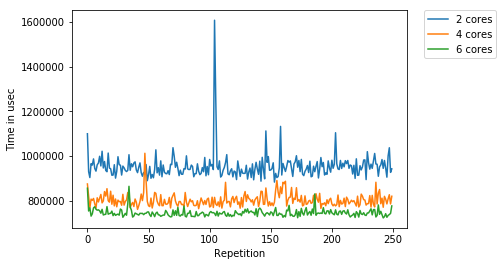
\includegraphics[scale=0.7]{images/colcpu.png}
    \caption{Benchmark im Columnstore unter Variation der CPU Kerne}\label{colcpu}}
\end{figure}


\autoref{colcpu} zeigt die Ausführungsdauer über den 250 Durchläufen des Benchmarks bei konstanten 8 Gigabyte RAM. Generell bewegt sich die Ausführungsdauer pro Benchmark hauptsächlich im Bereich von ca. 0.7 Sekunden bis 1 Sekunde. Dabei werden die schnelleren Werte, wie erwartet, durch den sechs-Kerner gebildet und die langsameren Werte durch den zwei-Kerner. Werden der sechs-Kerner(0.75 Sekunden) und der zwei-Kerner(0.95 Sekunden) anhand ihren arithmetischen Mitteln miteinander verglichen so ergibt sich eine prozentuale Differenz von 26.7\%. Der vier-Kerner hingegen erreicht eine durchschnittliche Ausführungszeit von 0,8 Sekunden was ihm eine Differenz von 7\% im Vergleich zum sechs-Kerner einbringt. 
Grundsätzlich gilt, dass im Columnstore im HANA Umfeld dank der begünstigten Parallelisierung eine bessere Ausnutzung der CPU durch mehrere Threads stattfindet. Dadurch wird die Nutzung der Hardware optimiert und eine bestmögliche Performance wird erzielt. Pro zusätzlichem Kern kann die Ausführungszeit halbiert werden, indem die Last gleichmäßig auf die Kerne aufgeteilt wird. Diese Überlegung stimmt mit den Messwerten überein und es lässt sich auf einen quadratischen Zuwachs der Ausführungszeit abhängig zur Anzahl der CPU-Kerne schliessen. 

\begin{figure}[H]
    \centering{
    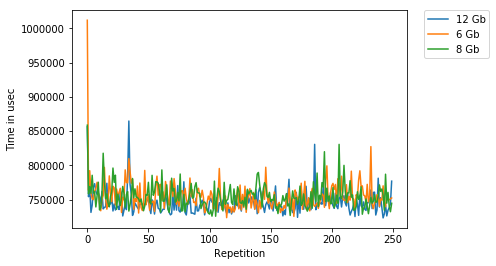
\includegraphics[scale=0.7]{images/colram.png}
    \caption{Benchmark im Columnstore unter Variation des RAMs}\label{colram}}
\end{figure}

\autoref{colram} zeigt die Ausführungsdauer über den 250 Durchläufen des Benchmarks bei konstanten 6 CPU Kernen. Die Ausführungsdauer pro Benchmark scheint nicht markant zu variieren, auch wenn die genauere Betrachtung der Aggregat-Werte zeigt, dass der Benchmark unter 12 Gigabyte RAM im Schnitt um eine Hunderdstel Sekunde schneller ist, als bei 6 und 8 Gigabyte. Ein besseres Mittel zum Vergleich als die Durchschnittslaufzeit bildet in diesem Falle die Standardabweichung der Laufzeiten, welche ein Maß für die Stabilität des Benchmarks darstellt. Diese beträgt bei 12 Gigabyte RAM gerade einmal 16 Millisekunden, während sich bei 8 Gigabyte ein 4 prozentiger Zuwachs und bei 6 Gigabyte ein 37 prozentiger Zuwachs erkennen lässt. Daraus lässt sich ableiten, dass die Stabilität stark unter der Einschränkung des RAMs leidet, und somit einzelne Anfragen erheblich länger dauern können. Vermutlich liegt die Unregelmäßigkeit vorallem darin begründet, dass bei reduziertem RAM externe Faktoren (Cache-Miss, Zugriffszeit) deutlicher zum tragen kommen. 

\subsection{Rowstore}

\begin{figure}[H]
    \centering{
    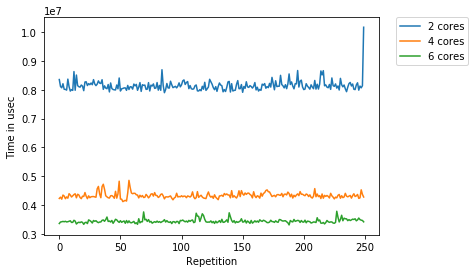
\includegraphics[scale=0.7]{images/rowcpu.png}
    \caption{Benchmark im Rowstore unter Variation der CPU Kerne}\label{rowcpu}}
\end{figure}

\autoref{rowcpu} zeigt die Ausführungsdauer über den 250 Durchläufen des Benchmarks bei konstanten 8 Gigabyte RAM. Zu erkennen ist die starke Abweichung der Ausführungszeiten, welcher deutlicher ausfällt als im Columnstore. Der zwei-Kerner liegt mit einer durschnittlichen Ausführungszeit von 8,2 Sekunden 137\% über der Ausführungszeit des acht-Kerners, welcher nur 3,4 Sekunden im Schnitt braucht. Die Abweichung des sechs-Kerners beträgt dagegen nur 26\%. 
Es scheint als würde die Anzahl der CPU-Kerne einen größeren Einfluss haben im Rowstore als im Columnstore. Eine mögliche Erklärung dafür kann folgendermaßen aussehen: 
Da die Daten im Columnstore blockweise gelesen werden können, haben die Lesezugriffe eine längere Ausführungszeit, da auch viele Daten in einem Zuge gelesen werden können. Der komplette Satz an Daten wird anschliessend von der CPU ausgewertet, wobei die Auswertung kürzer dauert als der Speicherzugriff. Dadurch wird das RAM zum Bottleneck und die CPU unrelevanter für die Ausführungszeit. 
Im Rowstore müssen viele einzelne Lesezugriffe durchgeführt werden, wobei die einzelnen Daten direkt verarbeitet werden von der CPU. Die Parallelität ist nicht in dem Maße gegeben wie im Columnstore, wodurch stets das RAM auf die CPU wartet und umgekehrt. Daraus ensteht eine erhöhte Relevanz der CPU für die Ausführungszeit als beim Columnstore. 

\begin{figure}[H]
    \centering{
    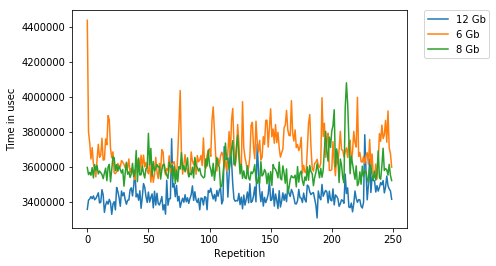
\includegraphics[scale=0.7]{images/rowram.png}
    \caption{Benchmark im Rowstore unter Variation des RAMs}\label{rowram}}
\end{figure}

\autoref{rowram} zeigt die Ausführungsdauer über den 250 Durchläufen des Benchmarks bei konstanten 6 CPU Kernen. Die Ausführungszeiten unterscheiden sich ebenfalls deutlicher als beim Columnstore. Unterschieden sich im Columstore die durchschnittlichen Ausführungszeiten von 12 Gigabyte und 6 Gigabyte RAM noch um 1,33\%, so liegt der Unterschied nun bereits bei 7,13\%. Die Standardabweichungen scheinen dasselbe Muster wie im Columnstore aufzuweisen: Je mehr RAM, desto stabiler läuft der Benchmark. Im Falle des 6 Gigabyte Systems sind enorme Ausschläge zu beobachten, obwohl teilweise sogar die Ausführungszeit des 8 Gigabyte Systems unterboten wird. 
Die erhöhte Relevanz der Menge an verfügbarem RAM scheint im Rowstore ebenfalls von größerer Bedeutung für die Laufzeit zu sein als im Columnstore. Während im Columnstore automatisch Optimierungen, wie Indexierung und Kompression stattfinden, können diese im Rowstore womöglich nur bei ausreichend RAM durchgeführt werden. 

\section{Vergleich zu anderen Datenbanksystemen}\label{auswertung:vergleich}

%TODO
%https://github.com/Osslack/HANA_SSBM/issues/27
%siehe auch ressourcen

